\section{Lepton reconstruction, selection and trigger efficiencies}\label{sec:Eff}

Since the lepton reconstruction, selection and trigger efficiencies can be slightly different between data and simulation,
correction factors have to be applied to the MC to account for these differences. The efficiencies are calculated using a Tag and Probe
technique exploiting Z boson decays to a pair of electrons or muons, respectively. One of the leptons is used as tag and has to pass a
tight selection, while the second one is used as probe if the tag-probe pair combines to the Z boson mass. The total lepton efficiency
can be factorized into three components:

\begin{equation}
\epsilon_{\textnormal{total}}=\epsilon_{\textnormal{Reco}}\cdot\epsilon_{\textnormal{Id}}\cdot\epsilon_{\textnormal{HLT}}
\end{equation}

The tag and probe method is nearly the same compared to the one already used in the 2011 data analysis for this Higgs search
(\cite{CMS-AN-12-029},\cite{CMS-AN-2012-021}). Therefore, only the most important information will be discussed.

\subsection{Electron efficiencies}\label{subsec:EffEle}
In the electron case, the reconstruction efficiency $\epsilon_{\textnormal{Reco}}$ characterizes the transition from a supercluster in the
electromagnetic calorimeter to a reconstructed Particle Flow electron. The ability of a reconstructed electron to pass the offline
selection consisting of several isolation and identification criteria is given by the identification efficiency $\epsilon_{\textnormal{Id}}$.
Finally, the selected electron has a certain probability to fire the high level trigger and the efficiency to fulfill the HLT requirements 
is parametrized as $\epsilon_{\textnormal{HLT}}$. In data, a single electron trigger is used at HLT level, while in MC the HLT requirements are dropped. \\
Since the HLT efficiency is MC is equal to $100\%$, the HLT efficiency measured on data is applied directly in the analysis of MC samples, 
while the other two efficiency components are calculated both for data and MC, so that a data/MC scale factor is applied in the other cases. \\
In general, since the efficiency depends both on $\pt$ and $\eta$ of the electron, the measurement is binned in $\pt$ as (30, 35, 40, 45, 50, 200)\GeVc 
and in $\eta$ as (-2.5, -1.5, 0.0, 1.5, 2.5) of the probe electron. The resulting efficiencies and scale factors are summarized in table~\ref{tab:eleEff} and
shown in figure~\ref{fig:eleEff}. 

\begin{table}[htb]
\centering 
\scalebox{0.70}{
  \begin{tabular}{|c|c|c|c|c|c|c|}
  \hline
  $p_{\textnormal{T,min}}$ & $p_{\textnormal{T,max}}$ & $\eta_{\textnormal{min}}$ & $\eta_{\textnormal{max}}$ & $\epsilon_{\textnormal{Reco,data}}$/$\epsilon_{\textnormal{Reco,mc}}$ & $\epsilon_{\textnormal{ID,data}}$/$\epsilon_{\textnormal{ID,mc}}$ & $\epsilon_{\textnormal{HLT,data}}$ \\
  $[\GeVc]$         & $[\GeVc]$         &                     &                     &                              &                           &                               \\
  \hline
  \hline
  30 & 35 & -2.5 & -1.5 & 1.000 $\pm$ 0.002 & 0.973 $\pm$ 0.004 & 0.639 $\pm$ 0.003 \\
  30 & 35 & -1.5 & 0 & 0.996 $\pm$ 0.001 & 0.981 $\pm$ 0.003 & 0.874 $\pm$ 0.001 \\
  30 & 35 & 0 & 1.5 & 0.996 $\pm$ 0.001 & 0.980 $\pm$ 0.003 & 0.874 $\pm$ 0.001 \\
  30 & 35 & 1.5 & 2.5 & 1.002 $\pm$ 0.001 & 0.999 $\pm$ 0.004 & 0.650 $\pm$ 0.003 \\
  35 & 40 & -2.5 & -1.5 & 1.001 $\pm$ 0.001 & 1.005 $\pm$ 0.003 & 0.686 $\pm$ 0.002 \\
  35 & 40 & -1.5 & 0 & 0.999 $\pm$ 0.001 & 0.978 $\pm$ 0.002 & 0.896 $\pm$ 0.001 \\
  35 & 40 & 0 & 1.5 & 0.998 $\pm$ 0.001 & 0.978 $\pm$ 0.002 & 0.891 $\pm$ 0.002 \\
  35 & 40 & 1.5 & 2.5 & 1.001 $\pm$ 0.001 & 1.003 $\pm$ 0.085 & 0.690 $\pm$ 0.002 \\
  40 & 45 & -2.5 & -1.5 & 1.001 $\pm$ 0.001 & 1.005 $\pm$ 0.003 & 0.708 $\pm$ 0.002 \\
  40 & 45 & -1.5 & 0 & 0.999 $\pm$ 0.001 & 0.985 $\pm$ 0.001 & 0.909 $\pm$ 0.001 \\
  40 & 45 & 0 & 1.5 & 0.999 $\pm$ 0.001 & 0.983 $\pm$ 0.001 & 0.906 $\pm$ 0.001 \\
  40 & 45 & 1.5 & 2.5 & 1.000 $\pm$ 0.001 & 1.014 $\pm$ 0.003 & 0.720 $\pm$ 0.002 \\
  45 & 50 & -2.5 & -1.5 & 1.001 $\pm$ 0.001 & 1.017 $\pm$ 0.003 & 0.724 $\pm$ 0.002 \\
  45 & 50 & -1.5 & 0 & 1.000 $\pm$ 0.001 & 0.984 $\pm$ 0.002 & 0.917 $\pm$ 0.001 \\
  45 & 50 & 0 & 1.5 & 0.999 $\pm$ 0.001 & 0.985 $\pm$ 0.002 & 0.911 $\pm$ 0.001 \\
  45 & 50 & 1.5 & 2.5 & 1.001 $\pm$ 0.001 & 1.021 $\pm$ 0.003 & 0.733 $\pm$ 0.002 \\
  50 & 200 & -2.5 & -1.5 & 0.999 $\pm$ 0.001 & 1.023 $\pm$ 0.003 & 0.733 $\pm$ 0.003 \\
  50 & 200 & -1.5 & 0 & 0.999 $\pm$ 0.001 & 0.990 $\pm$ 0.002 & 0.925 $\pm$ 0.001 \\
  50 & 200 & 0 & 1.5 & 0.999 $\pm$ 0.001 & 0.991 $\pm$ 0.003 & 0.920 $\pm$ 0.001 \\
  50 & 200 & 1.5 & 2.5 & 1.000 $\pm$ 0.001 & 1.019 $\pm$ 0.003 & 0.745 $\pm$ 0.003 \\
  \hline
  \end{tabular}}
\caption{Electron efficiency and data/MC scale factors for super-cluster to reconstructed electrons ($\epsilon_{\textnormal{Reco}}$),
    reconstructed to selected electrons ($\epsilon_{\textnormal{ID}}$) and selected to HLT electrons ($\epsilon_{\textnormal{HLT}}$). 
    The errors are statistical only.} 
\label{tab:eleEff} 
\end{table}

\begin{figure}[b]
  \begin{center}
    \subfigure[]{
    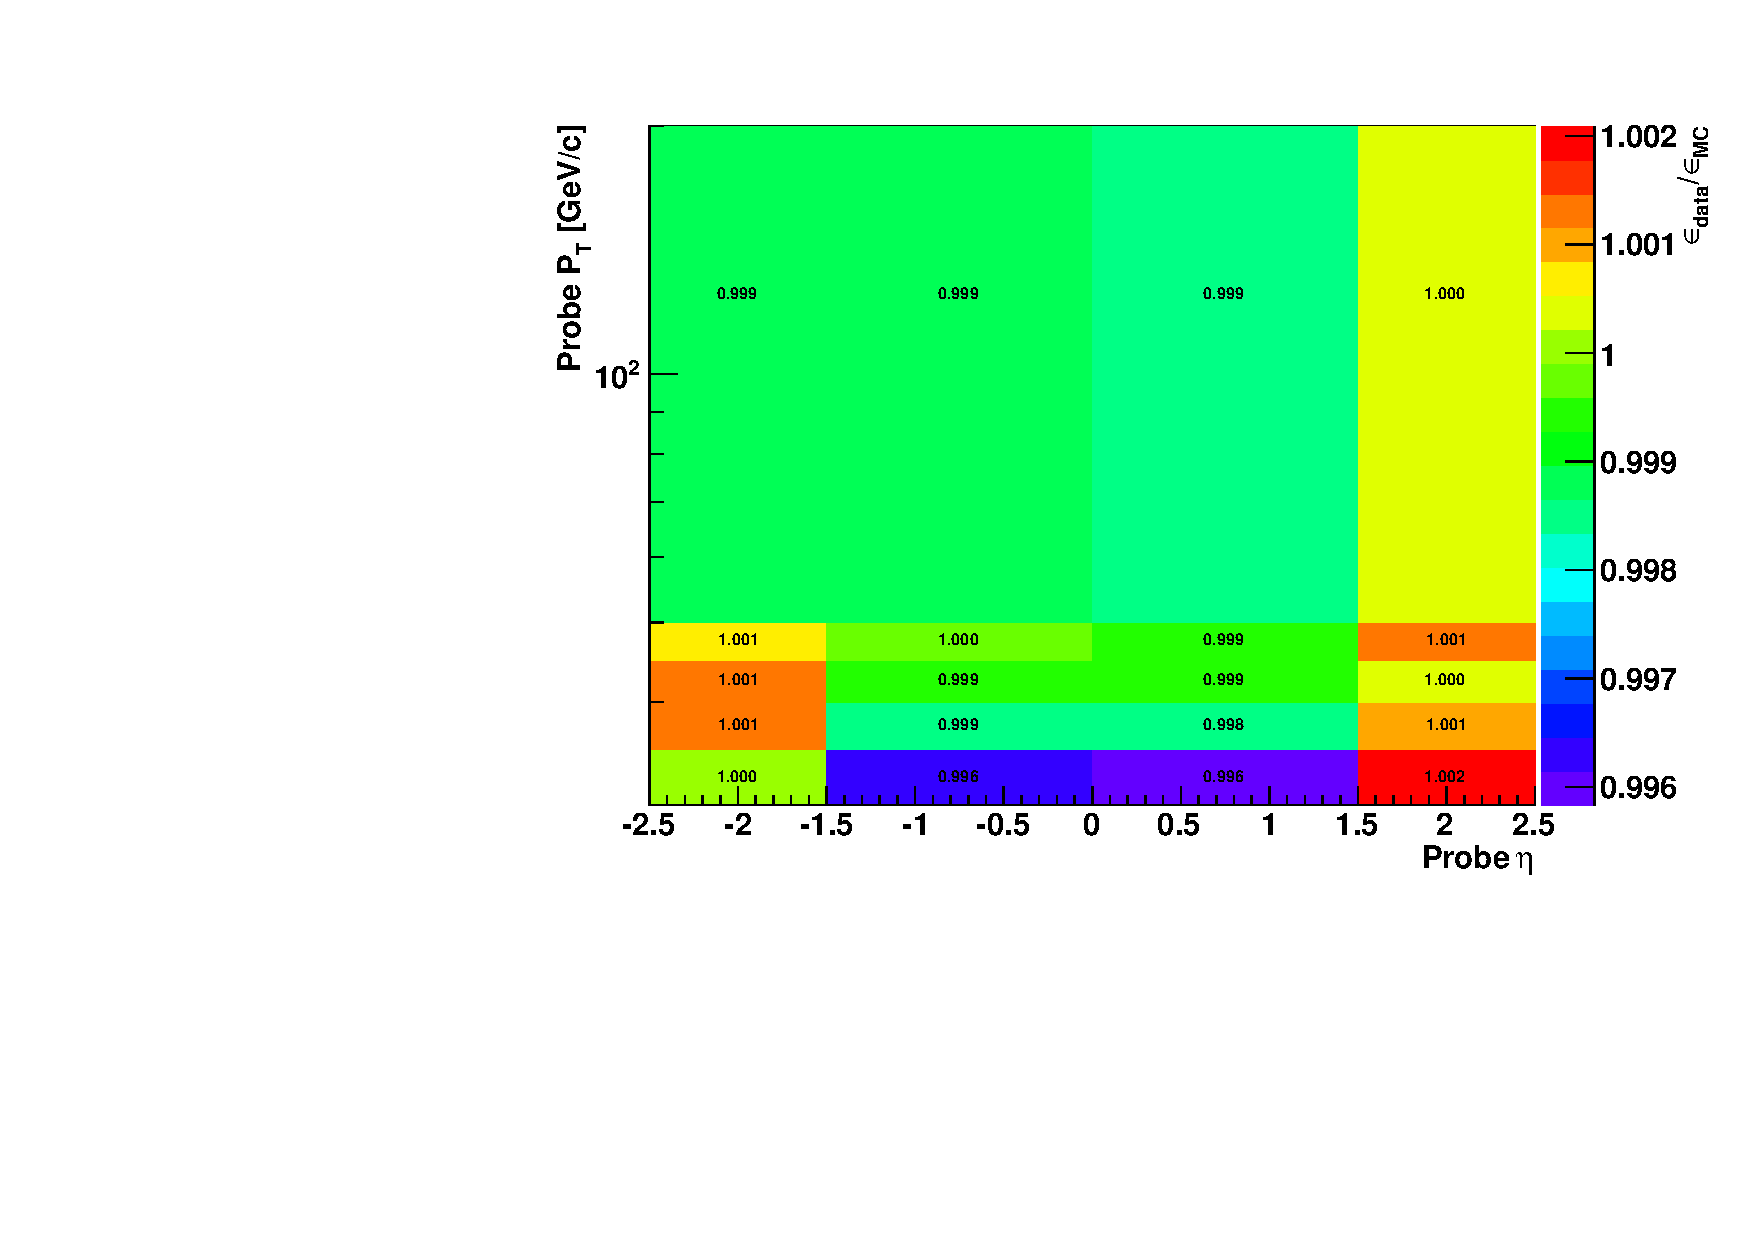
\includegraphics[width=0.32\textwidth]{plots/scaleFactor-Run2012ABC-SCToElectron.pdf}
  }
    \subfigure[]{
    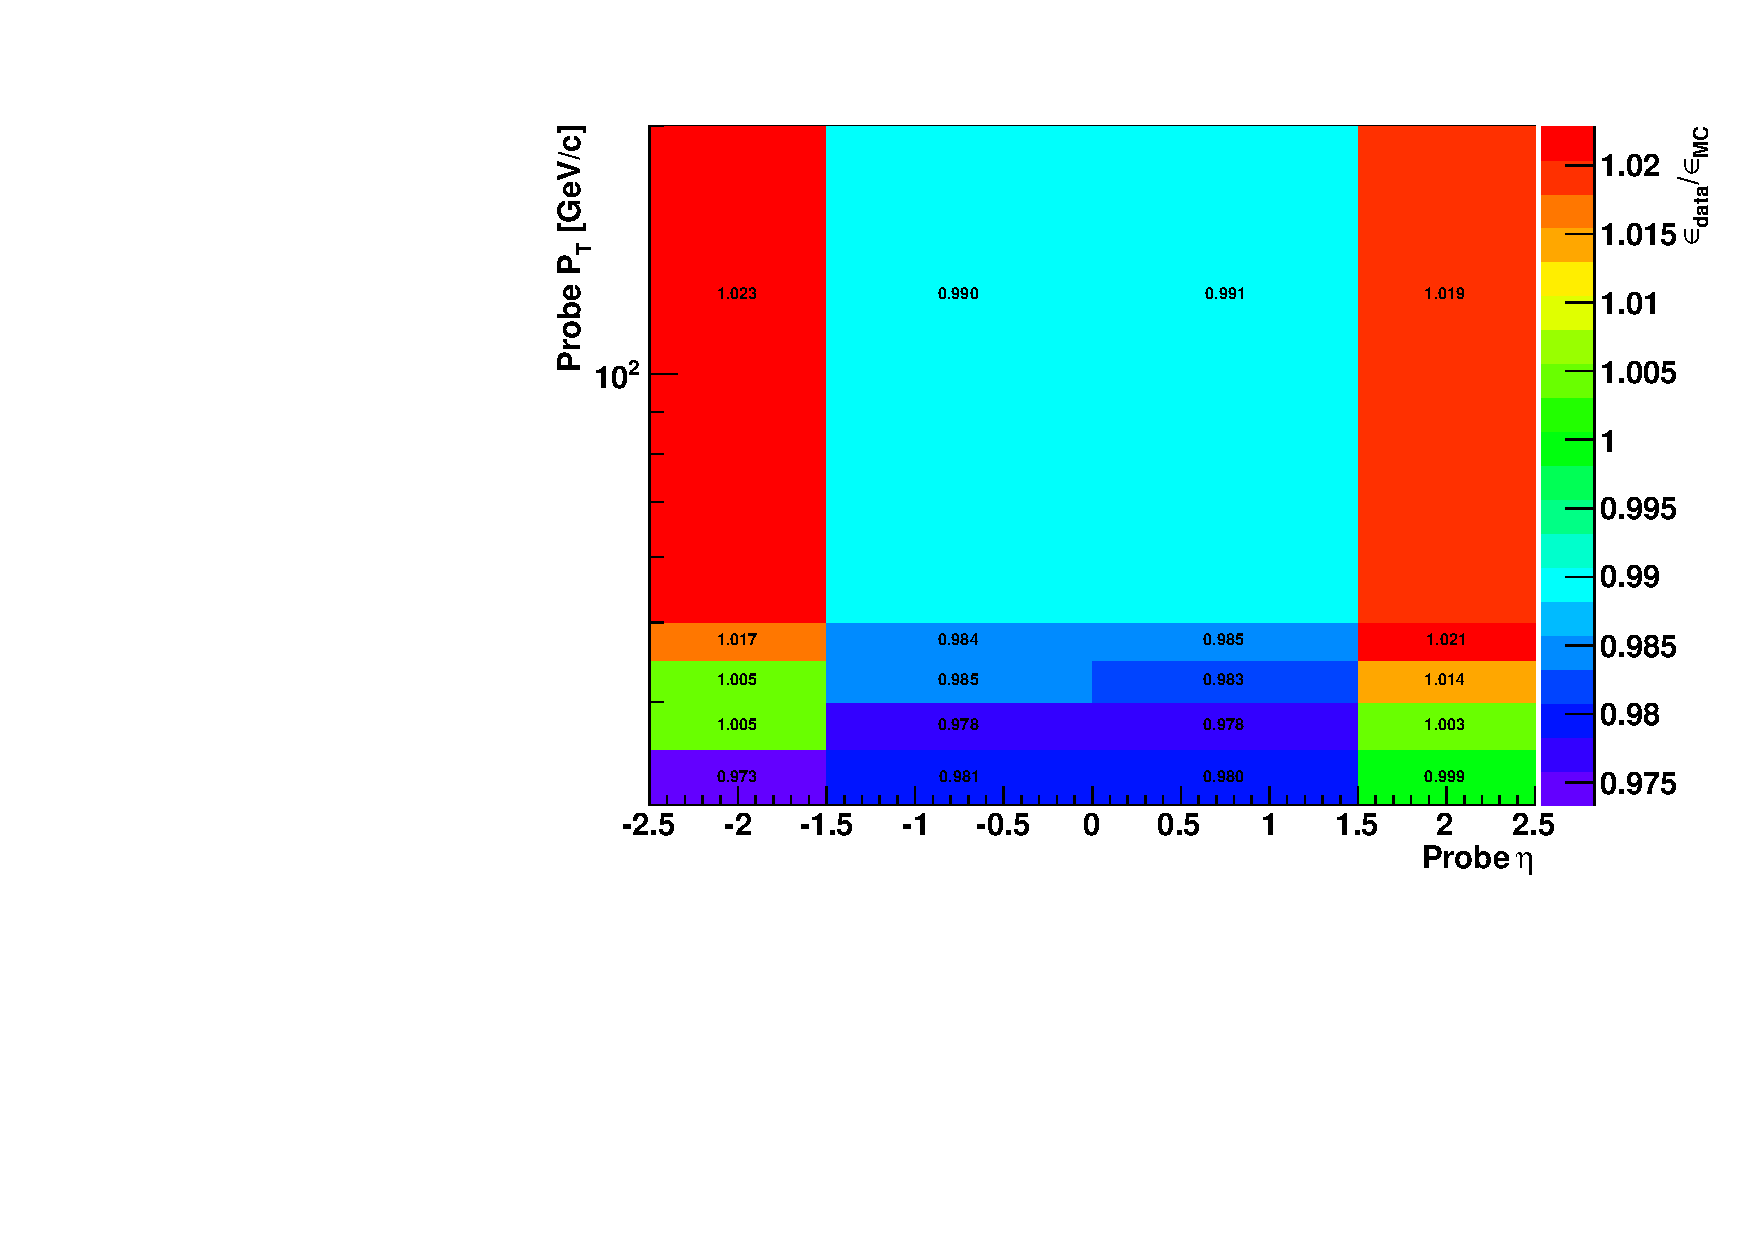
\includegraphics[width=0.32\textwidth]{plots/scaleFactor-Run2012ABC-GsfElectronToId.pdf}
  }
  \subfigure[]{
    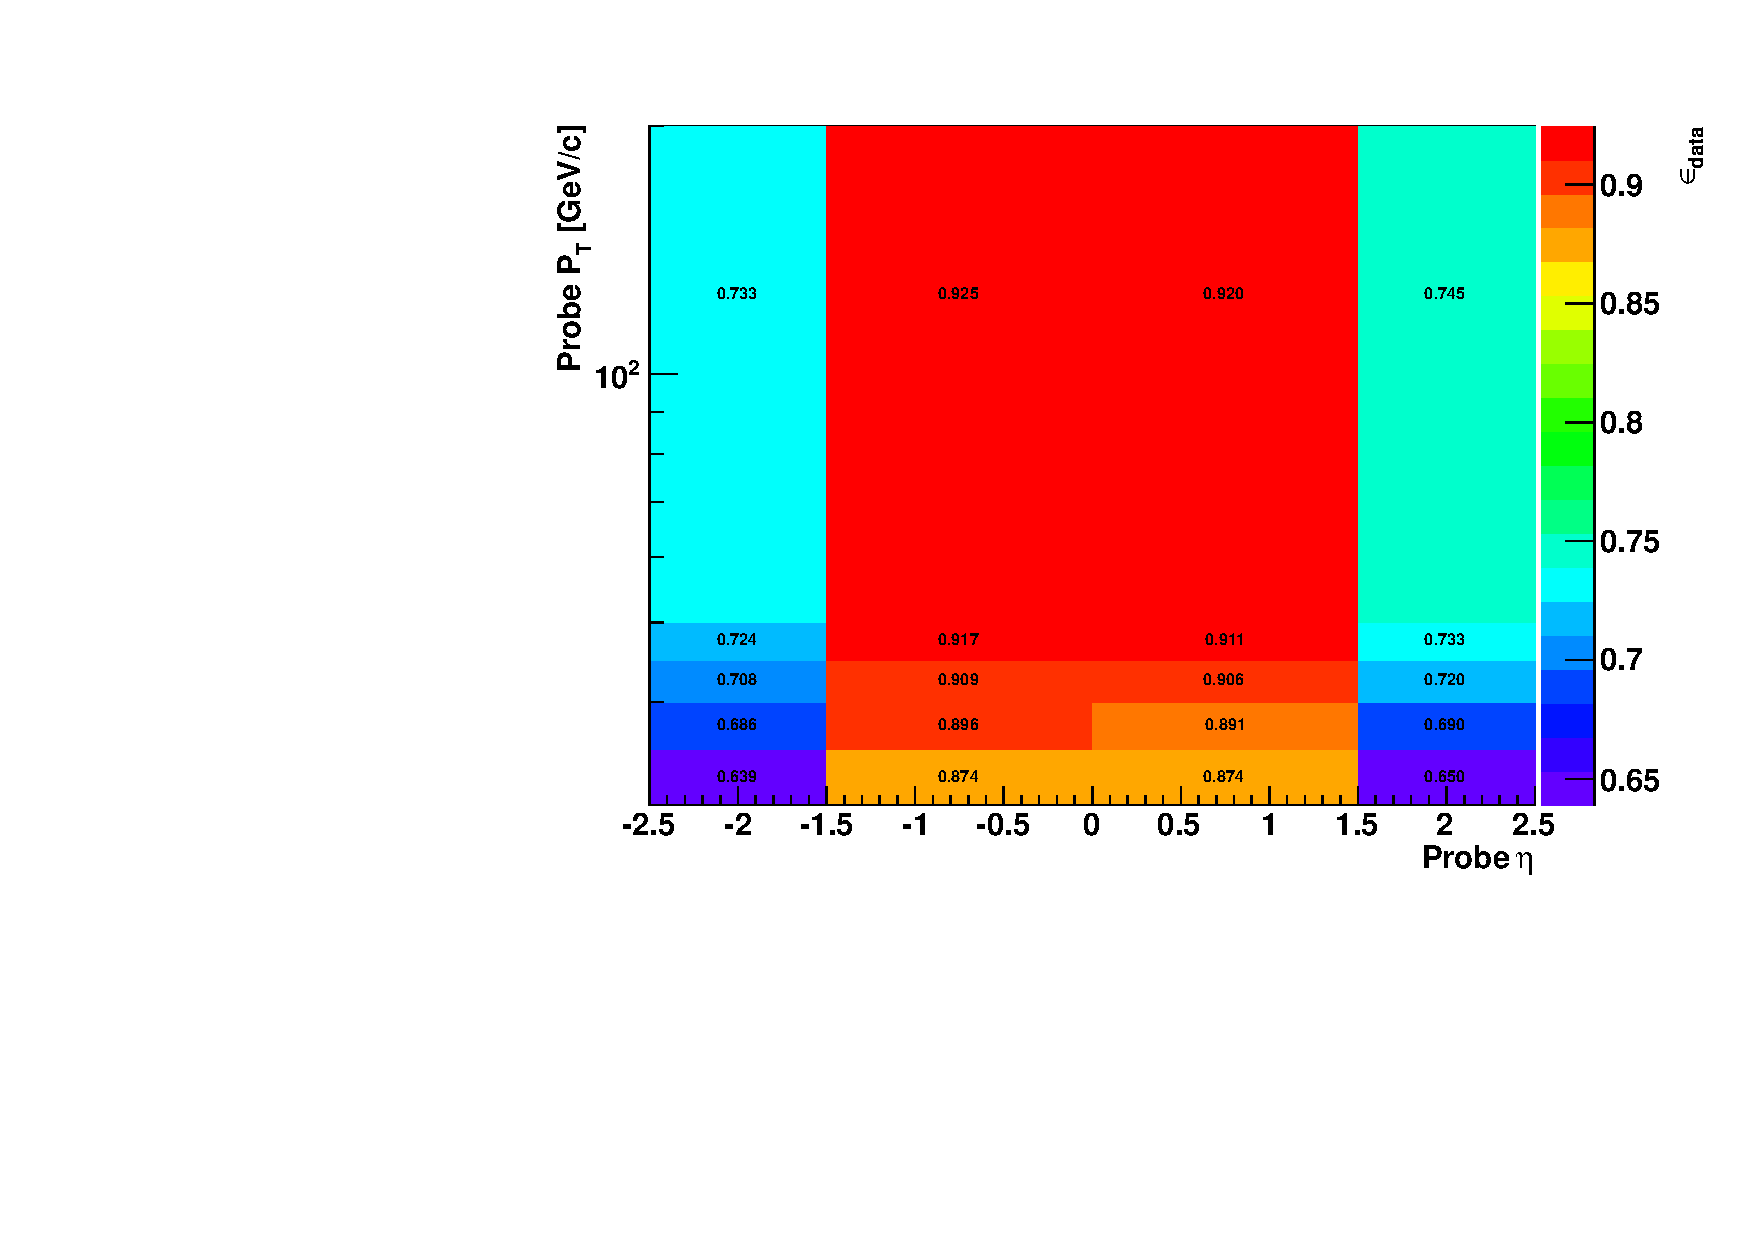
\includegraphics[width=0.32\textwidth]{plots/efficiency-Run2012ABC-WP80ToHLTEle.pdf}
  }
    \caption{Electron efficiency and data/MC scale factors for super-cluster to reconstructed electrons $\epsilon_{\textnormal{Reco}}$ (a),
    reconstructed to selected electrons $\epsilon_{\textnormal{Id}}$ (b) and selected to HLT electrons
      $\epsilon_{\textnormal{HLT}}$ (c).}
    \label{fig:eleEff}
  \end{center}
\end{figure}

\subsection{Muon efficiencies}\label{subsec:EffMu}

In the muon case, the reconstruction efficiency $\epsilon_{\textnormal{Reco}}$ describes the ability to reconstruct a Particle Flow muon starting with
a particle track and can be assumed to be one \cite{MUONPAS}. The identification efficiency $\epsilon_{\textnormal{Id}}$ gives an estimate for a
reconstructed muon to pass the offline selection criteria. It can be computed for both data and simulation and thus a scale factor being
the ratio of the two efficiencies is derived. \\
The trigger efficiency $\epsilon_{\textnormal{HLT}}$  is the fraction of selected muons fulfilling the HLT requirements and, since the HLT
requirement is dropped on the MC analysis, the efficiency computed on data is used directly to correct the MC event expectation.\\
The efficiency measurement is binned both in $\pt$ and $\eta$ of the probe muon covering the
relevant intervals (25, 30, 35, 40, 45, 50, 200)\GeVc in $\pt$ and (-2.1, -1.5, -1.0, -0.5, 0.0, 0.5, 1.0, 1.5, 2.1) in $\eta$. The resulting selection
and trigger efficiencies and scale factors are summarized in table~\ref{tab:muonEff} and figure~\ref{fig:muonEff}.

\begin{table}[htb]
\centering 
\scalebox{0.70}{
  \begin{tabular}{|c|c|c|c|c|c|}
  \hline
  $p_{\textnormal{T,min}}$ & $p_{\textnormal{T,max}}$ & $\eta_{\textnormal{min}}$ & $\eta_{\textnormal{max}}$ & $\epsilon_{\textnormal{ID,data}}$/$\epsilon_{\textnormal{ID,mc}}$ & $\epsilon_{\textnormal{HLT,data}}$ \\
  $[\GeVc]$         & $[\GeVc]$         &                     &                     &                             &                               \\
  \hline
  \hline
  25 & 30 & -2.1 & -1.5 & 0.992 $\pm$ 0.003 & 0.766 $\pm$ 0.003 \\
  25 & 30 & -1.5 & -1 & 0.987 $\pm$ 0.003 & 0.822 $\pm$ 0.003 \\
  25 & 30 & -1 & -0.5 & 0.990 $\pm$ 0.003 & 0.914 $\pm$ 0.002 \\
  25 & 30 & -0.5 & 0 & 0.984 $\pm$ 0.003 & 0.920 $\pm$ 0.002 \\
  25 & 30 & 0 & 0.5 & 0.985 $\pm$ 0.003 & 0.924 $\pm$ 0.002 \\
  25 & 30 & 0.5 & 1 & 0.992 $\pm$ 0.003 & 0.913 $\pm$ 0.002 \\
  25 & 30 & 1 & 1.5 & 0.991 $\pm$ 0.003 & 0.802 $\pm$ 0.003 \\
  25 & 30 & 1.5 & 2.1 & 0.995 $\pm$ 0.002 & 0.814 $\pm$ 0.003 \\
  30 & 35 & -2.1 & -1.5 & 0.991 $\pm$ 0.002 & 0.785 $\pm$ 0.002 \\
  30 & 35 & -1.5 & -1 & 0.988 $\pm$ 0.002 & 0.829 $\pm$ 0.002 \\
  30 & 35 & -1 & -0.5 & 0.988 $\pm$ 0.002 & 0.921 $\pm$ 0.002 \\
  30 & 35 & -0.5 & 0 & 0.984 $\pm$ 0.002 & 0.930 $\pm$ 0.001 \\
  30 & 35 & 0 & 0.5 & 0.985 $\pm$ 0.002 & 0.935 $\pm$ 0.001 \\
  30 & 35 & 0.5 & 1 & 0.990 $\pm$ 0.002 & 0.922 $\pm$ 0.002 \\
  30 & 35 & 1 & 1.5 & 0.987 $\pm$ 0.002 & 0.807 $\pm$ 0.002 \\
  30 & 35 & 1.5 & 2.1 & 0.995 $\pm$ 0.002 & 0.833 $\pm$ 0.002 \\
  35 & 40 & -2.1 & -1.5 & 0.992 $\pm$ 0.002 & 0.793 $\pm$ 0.002 \\
  35 & 40 & -1.5 & -1 & 0.987 $\pm$ 0.002 & 0.832 $\pm$ 0.002 \\
  35 & 40 & -1 & -0.5 & 0.991 $\pm$ 0.002 & 0.926 $\pm$ 0.001 \\
  35 & 40 & -0.5 & 0 & 0.986 $\pm$ 0.002 & 0.935 $\pm$ 0.001 \\
  35 & 40 & 0 & 0.5 & 0.986 $\pm$ 0.002 & 0.940 $\pm$ 0.001 \\
  35 & 40 & 0.5 & 1 & 0.991 $\pm$ 0.002 & 0.925 $\pm$ 0.001 \\
  35 & 40 & 1 & 1.5 & 0.989 $\pm$ 0.002 & 0.812 $\pm$ 0.002 \\
  35 & 40 & 1.5 & 2.1 & 0.994 $\pm$ 0.002 & 0.837 $\pm$ 0.002 \\
  40 & 45 & -2.1 & -1.5 & 0.994 $\pm$ 0.002 & 0.800 $\pm$ 0.002 \\
  40 & 45 & -1.5 & -1 & 0.987 $\pm$ 0.001 & 0.837 $\pm$ 0.002 \\
  40 & 45 & -1 & -0.5 & 0.992 $\pm$ 0.001 & 0.927 $\pm$ 0.001 \\
  40 & 45 & -0.5 & 0 & 0.986 $\pm$ 0.001 & 0.940 $\pm$ 0.001 \\
  40 & 45 & 0 & 0.5 & 0.987 $\pm$ 0.001 & 0.944 $\pm$ 0.001 \\
  40 & 45 & 0.5 & 1 & 0.991 $\pm$ 0.001 & 0.928 $\pm$ 0.001 \\
  40 & 45 & 1 & 1.5 & 0.991 $\pm$ 0.001 & 0.817 $\pm$ 0.002 \\
  40 & 45 & 1.5 & 2.1 & 0.996 $\pm$ 0.001 & 0.844 $\pm$ 0.002 \\
  45 & 50 & -2.1 & -1.5 & 0.993 $\pm$ 0.002 & 0.807 $\pm$ 0.002 \\
  45 & 50 & -1.5 & -1 & 0.987 $\pm$ 0.002 & 0.840 $\pm$ 0.002 \\
  45 & 50 & -1 & -0.5 & 0.990 $\pm$ 0.001 & 0.931 $\pm$ 0.001 \\
  45 & 50 & -0.5 & 0 & 0.988 $\pm$ 0.002 & 0.941 $\pm$ 0.001 \\
  45 & 50 & 0 & 0.5 & 0.987 $\pm$ 0.002 & 0.947 $\pm$ 0.001 \\
  45 & 50 & 0.5 & 1 & 0.992 $\pm$ 0.001 & 0.930 $\pm$ 0.001 \\
  45 & 50 & 1 & 1.5 & 0.991 $\pm$ 0.002 & 0.821 $\pm$ 0.002 \\
  45 & 50 & 1.5 & 2.1 & 0.995 $\pm$ 0.002 & 0.851 $\pm$ 0.002 \\
  50 & 200 & -2.1 & -1.5 & 0.991 $\pm$ 0.002 & 0.809 $\pm$ 0.002 \\
  50 & 200 & -1.5 & -1 & 0.987 $\pm$ 0.002 & 0.842 $\pm$ 0.002 \\
  50 & 200 & -1 & -0.5 & 0.992 $\pm$ 0.002 & 0.931 $\pm$ 0.001 \\
  50 & 200 & -0.5 & 0 & 0.987 $\pm$ 0.002 & 0.944 $\pm$ 0.001 \\
  50 & 200 & 0 & 0.5 & 0.989 $\pm$ 0.002 & 0.946 $\pm$ 0.001 \\
  50 & 200 & 0.5 & 1 & 0.992 $\pm$ 0.002 & 0.932 $\pm$ 0.001 \\
  50 & 200 & 1 & 1.5 & 0.993 $\pm$ 0.002 & 0.824 $\pm$ 0.002 \\
  50 & 200 & 1.5 & 2.1 & 0.996 $\pm$ 0.002 & 0.854 $\pm$ 0.002 \\
  \hline
  \end{tabular}}
\caption{Muon selection scale factors and HLT efficiencies. The errors are statistical only.} 
\label{tab:muonEff} 
\end{table}

\begin{figure}[t]
  \begin{center}
    \subfigure[]{
    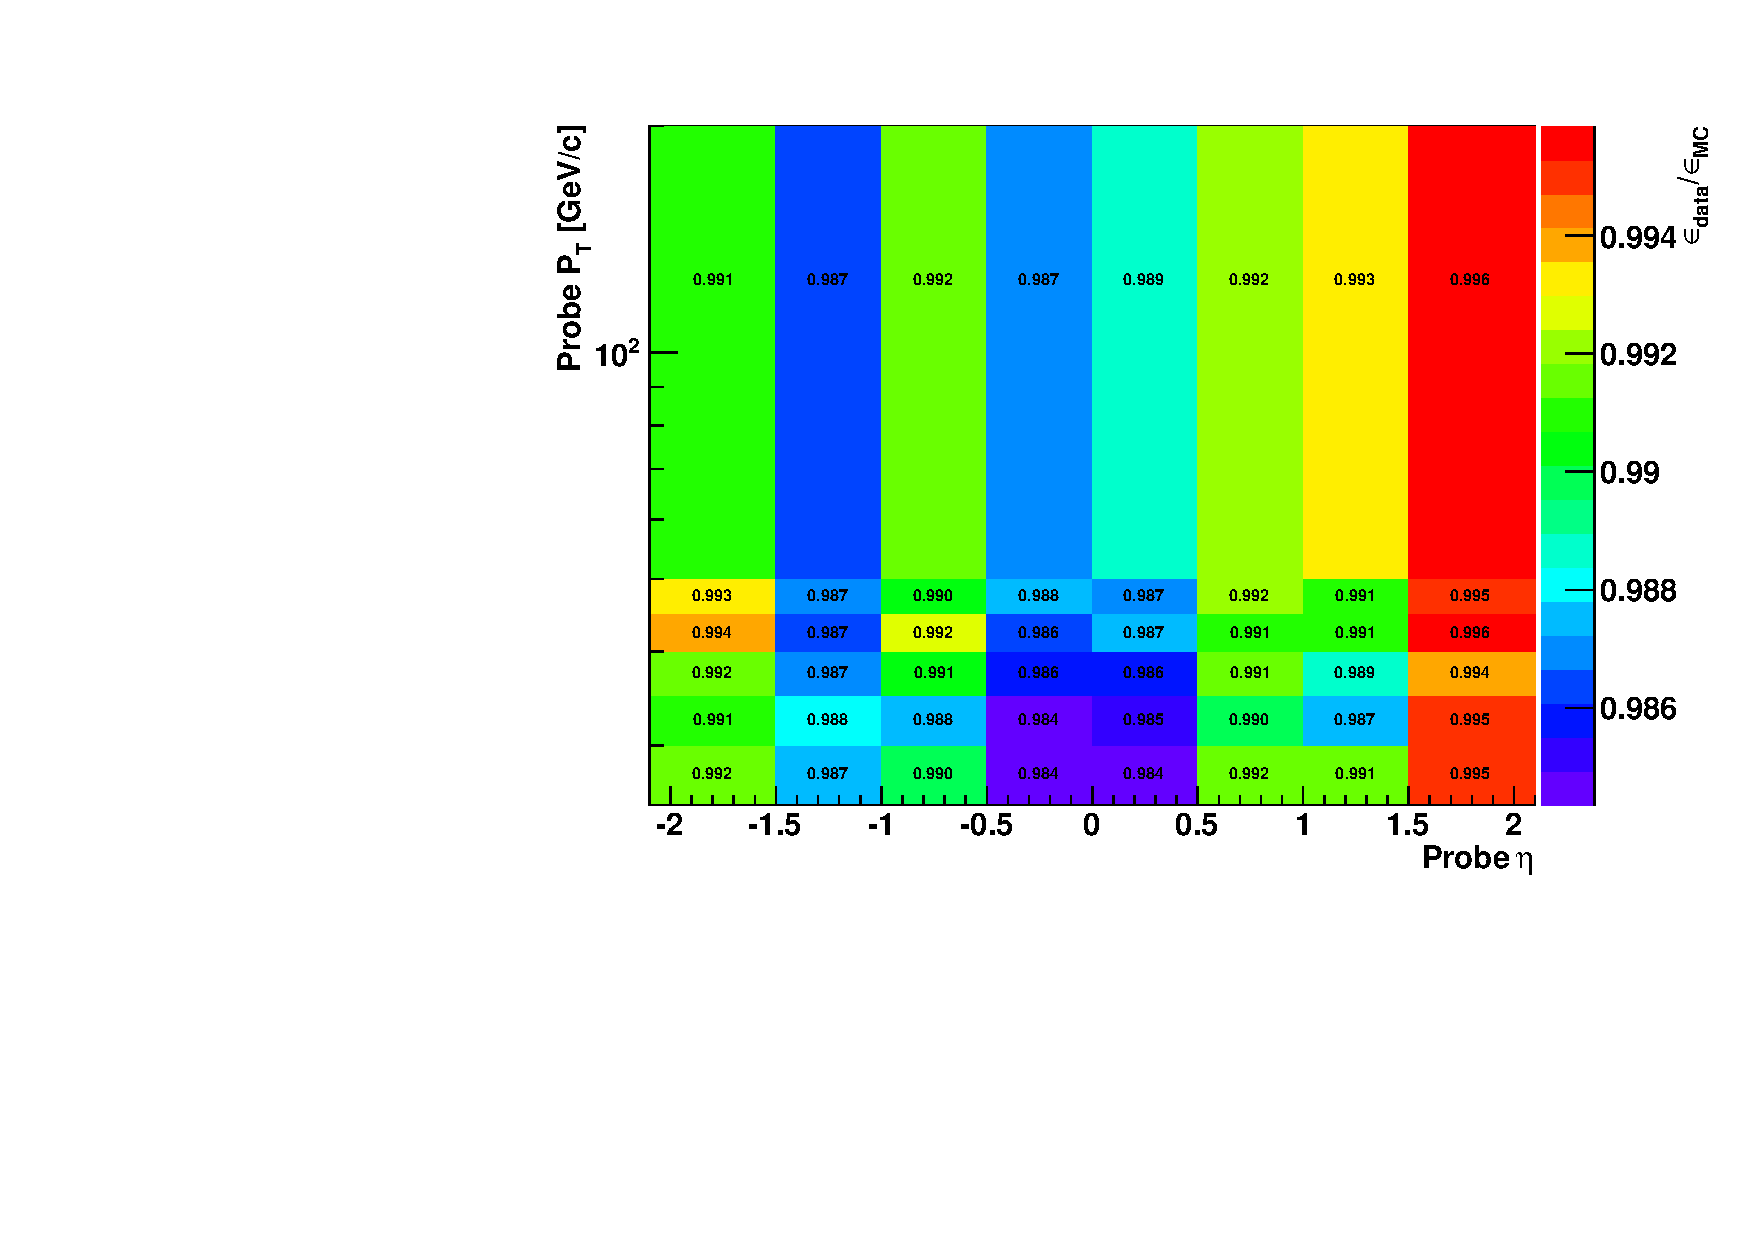
\includegraphics[width=0.47\textwidth]{plots/scaleFactor-Run2012ABC-RecoToIso.pdf}
  }
  \subfigure[]{
    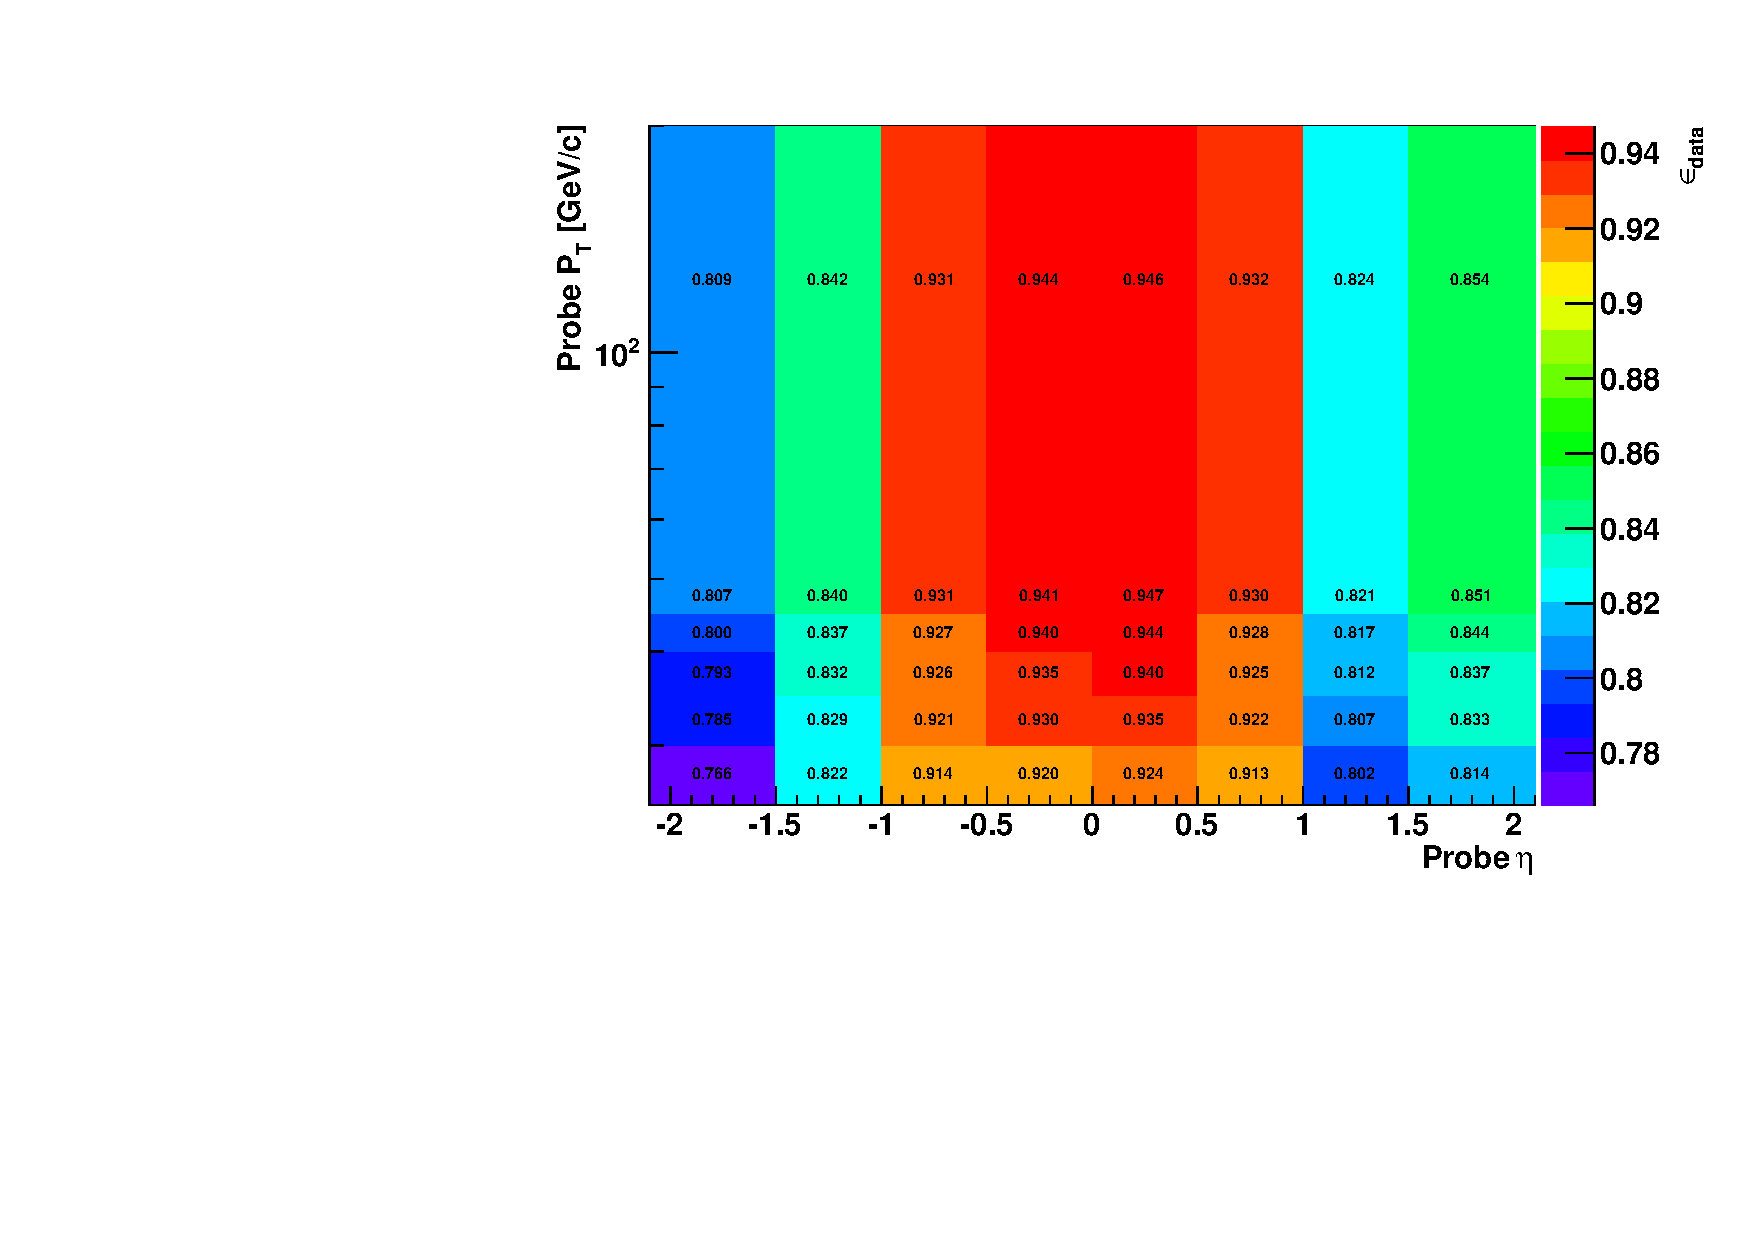
\includegraphics[width=0.47\textwidth]{plots/efficiency-Run2012ABC-IsoToIsoMuHLT.pdf}
  }
    \caption{Muon scale factors for reconstructed to selected muons $\epsilon_{\textnormal{ID,data}}$/$\epsilon_{\textnormal{ID,mc}}$ (a) and 
    efficiency for selected to HLT muons $\epsilon_{\textnormal{HLT,data}}$ (b).}
    \label{fig:muonEff}
  \end{center}
\end{figure}